\documentclass{lab_sheet}
\usepackage{pgfplots}
\usepackage{tikz}
\usepackage{wrapfig}
\usetikzlibrary{decorations.pathreplacing}
\pgfplotsset{compat=newest}
\begin{document}
    \titlePage{Detection and Demodulation of AM Signal}{February 8, 2021}
    \pagenumbering{gobble}
    \tableofcontents
    \pagebreak
    \pagenumbering{arabic}
    \section{Objectives}
    \begin{itemize}
        \item To recover original modulation signal from the transmitted DSB
        \item To observe diagonal peak clipping and negative peak clipping occurring in AM detection
     \end{itemize}
    \section{Required Tools}
    \begin{itemize}
        \item Signal generator
        \item Double beam digital oscilloscope
        \item ED-2900P, ED-2950D and ED-2960D
        \item Envelope detector
        \item Signal processing and wireless communications MATLAB application modules
    \end{itemize}
\section{Introduction}
\subsection{Demodulation of AM Signals}
Demodulation is somewhat the reverse of modulation of signals, where modulated signals are demodulated to retrive the true information after transmission. Demodulation is a key process in the reception of any amplitude modulated signals. Demodulation is the process by which the original information bearing signal, i.e. the modulation is extracted from the incoming overall received signal. The process of demodulation for signals using amplitude modulation can be achieved in a number of different techniques, viz. Square law demodulator and Envelope detector. The lab experiment deals with the envelope detector method to demodulate an AM signal.
\subsection{Envelope Detector}
Envelope detector is one of the most common circuits that produces output voltage that is proportional to the envelope of the input signal. 
\begin{figure}[H]
    \centering
    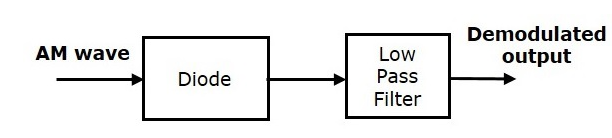
\includegraphics{Figures/env.png}
    \caption{Block diagram for demodulation of AM signal using a diode envelope detector}
    \label{fig:env}
\end{figure}
An envelope detector is actually a half-wave rectifier that charges a capacitor to the peak voltage of the incoming AM signal. When the input signal’s amplitude increases, the capacitor charges via the rectifying diode. When the input's amplitude falls, the capacitor voltage is reduced
by being discharged through a the discharge resistor, R.
\begin{figure}[H]
    \centering
    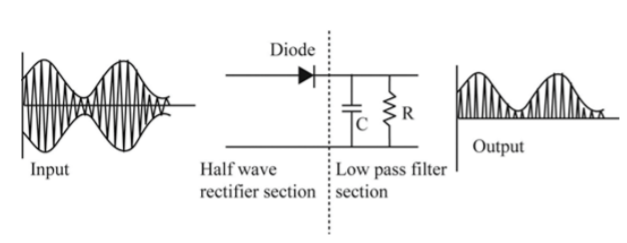
\includegraphics{Figures/env2.png}
    \caption{Circuit diagram for demodulation of AM signal using a diode envelope detector}
    \label{fig:env2}
\end{figure}
It is widely used in demodulation of AM signals since it is a low cost circuit with minimum components and is quite simple to implement.
\subsubsection{Practical Issues} 
\subsubsection*{Dependency on Ideal Characteristics of Diode}
Since all practical diodes exhibit non-linear IV characteristics, the demodulated signal from the circuit using the diode as a switch also reflects the non-linear characteristics.
\subsubsection*{Ripple Effect}
When the capacitor in the filter circuit discharges faster than it is supposed to, ripple is seen in the signal. Consider a carrier frequency $f_c$ and an envelope detector with time constant $\tau=RC$. Then, the succesive peaks of the carrier occur after $T=\frac{1}{f_c}$.
\\
For $\tau >> T$, the capacitor discharges from the peak voltage $V_{peak}$ to $V'$ as, $$V'=V_{peak}\left(1-\frac{T}{\tau}\right)$$Thus, the peak-to-peak size of ripple, $\Delta V$ is calculated as,
$$\Delta V=\frac{V_{peak}T}{\tau}=\frac{V_{peak}}{f_c \tau}$$
\subsubsection*{Negative Peak Clipping}
When the capacitor is unable to discharge as quickly as it is supposed to, negative peak clipping occurs. To visualize the effect, consider a square wave as the modulating signal for a sine carrier signal. In such case, the capacitor won't discharge fast enough to track the signal envelope which results in the negative peak being clipped. \\
To reduce the effect of negative peak clipping, the following relation must be followed while choosing a capacitor,
$$
\frac{1}{f_c}>>\tau>>\frac{1}{f_m}
$$
\begin{figure}[H]
    \centering
    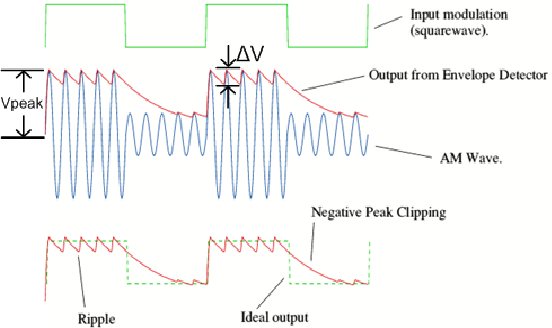
\includegraphics[scale=0.8]{Figures/negclip.png}
    \caption{Ripple effect and negative peak clipping in an envelope detector}
    \label{fig:neg}
\end{figure}
\section{Lab Experiment Observations}
Modulating signal frequency ($f_m$) = 377 KHz\\
Carrier signal frequency ($f_c$) = 480 MHz 

\begin{figure}[H]
    \centering
    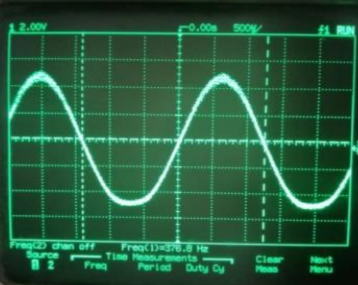
\includegraphics[scale=1.2]{Figures/demod.png}
    \caption{Demodulated signal for under modulation}
    \label{fig:demod}
\end{figure}

\begin{figure}[H]
    \centering
    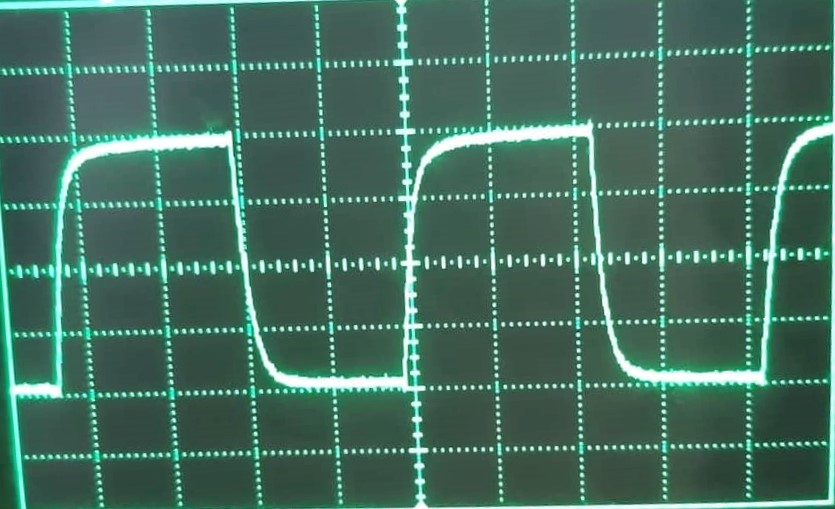
\includegraphics[scale=0.4]{Figures/perf_mod.jpg}
    \caption{Demodulated signal for perfect modulation}
    \label{fig:perf}
\end{figure}

    \begin{figure}[H]
        \centering
        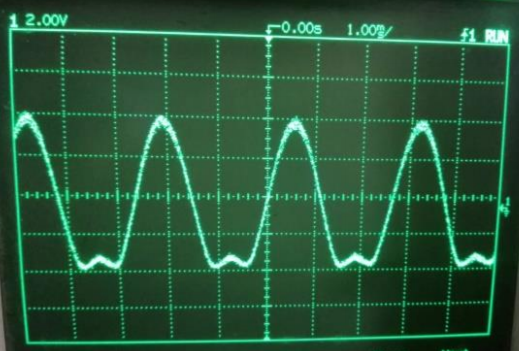
\includegraphics[scale=0.85]{Figures/distorted.png}
        \caption{Distorted demodulated signal for over modulation}
        \label{fig:dist}
    \end{figure}

    \section{MATLAB Script for Demodulation using Envelope Detector}
    \matlabcode{demod}{Demodulation using Envelope Detector}
    \section{Simulated Signal Observation}
    \begin{figure}[H]
        \centering
        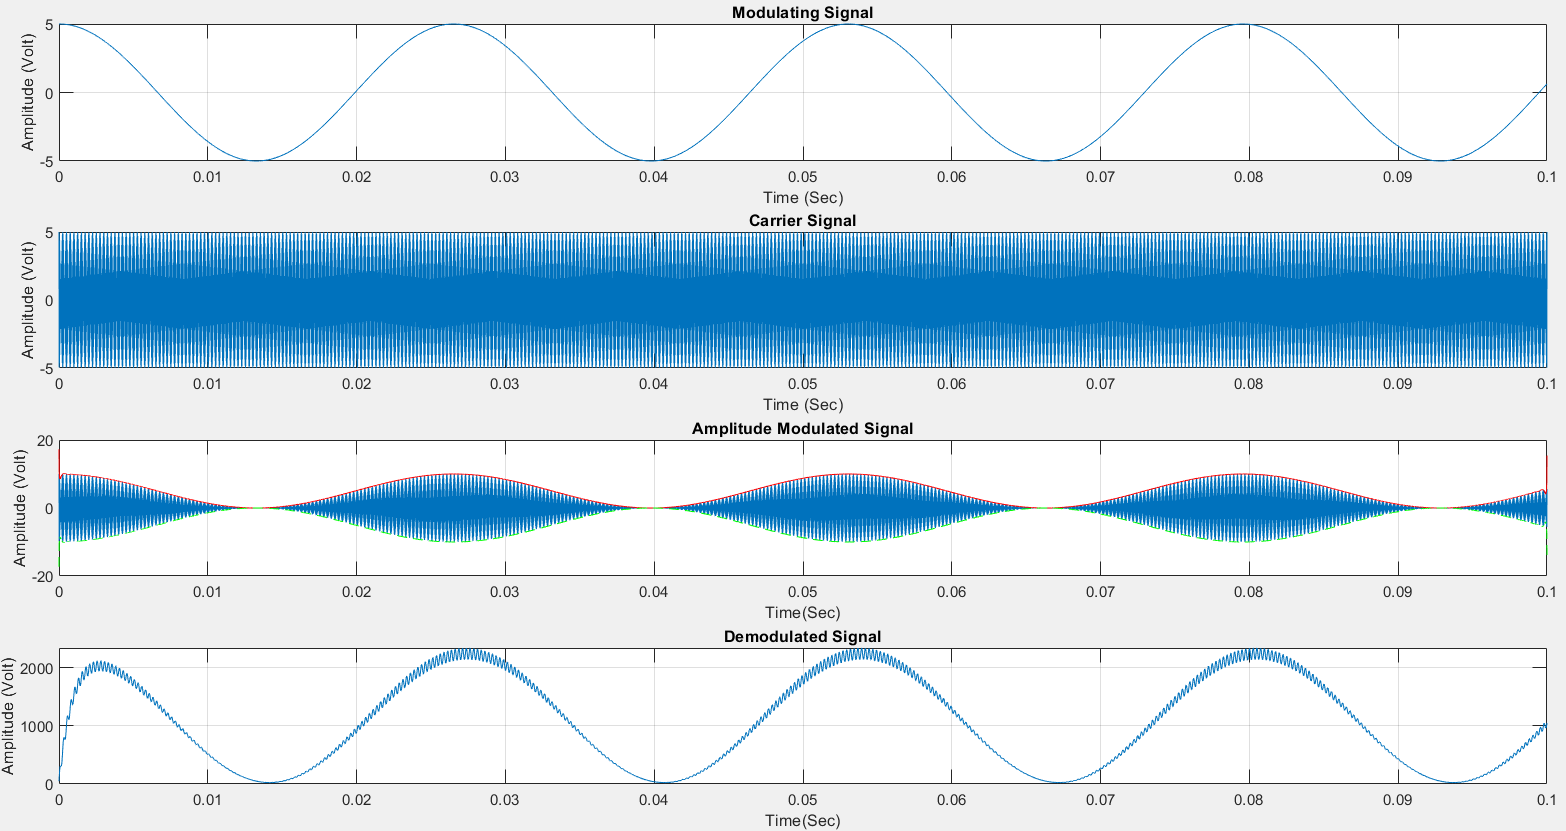
\includegraphics[width=\linewidth]{Figures/sim_demod.png}
        \caption{Demodulated signal generated from envelope detector}
        \label{fig:simdemod}
    \end{figure}
    \section{Discussion and Conclusion}
    The lab experiment dealt with the basic concept of amplitude demodulation to get the original message signal from an AM signal. During the lab experiment, message signal with frequnecy, $f_m=377$ KHz and carrier signal with frequency, $f_c=480$ MHz were generated using the signal generator. With the use of a balanced modulator, DSB-FC amplitude modulated signal was generated. This was then supplied to the envelope detector that produced demodulated signals which were visualized using the oscilloscope.
    It was observed that for under modulation, the output signal from the envelope was approximately identical to the original message signal in addition to the ripples observed. The resulting demodulated signal from a perfectly modulated AM signal was observed to have flat peaks due to leveling at zero crossing. Likewise, distortion was visible in case of over modulated signal which is a result of small crests being followed by the envelope detector.\\To gain more perspective on AM demodulation, MATLAB script for generation of an AM signal, calculation of it's envelope signals and finally demodulation is also included in this report.\\
    This lab allowed us to visualize the amplitude demodulation using an envelope detector. Hence, the objectives of the lab experiment are fulfilled. 
\end{document}